%%
%% This is file `sigconf.tex',
%% generated with the docstrip utility.
%%
%% The original source files were:
%%
%% samples.dtx  (with options: `all,proceedings,sigconf')
%% 
%% IMPORTANT NOTICE:
%% 
%% For the copyright see the source file.
%% 
%% Any modified versions of this file must be renamed
%% with new filenames distinct from sigconf.tex.
%% 
%% For distribution of the original source see the terms
%% for copying and modification in the file samples.dtx.
%% 
%% This generated file may be distributed as long as the
%% original source files, as listed above, are part of the
%% same distribution. (The sources need not necessarily be
%% in the same archive or directory.)
%%
%%
%% Commands for TeXCount
%TC:macro \cite [option:text,text]
%TC:macro \citep [option:text,text]
%TC:macro \citet [option:text,text]
%TC:envir table 0 1
%TC:envir table* 0 1
%TC:envir tabular [ignore] word
%TC:envir displaymath 0 word
%TC:envir math 0 word
%TC:envir comment 0 0
%%
%% The first command in your LaTeX source must be the \documentclass
%% command.
%%
%% For submission and review of your manuscript please change the
%% command to \documentclass[manuscript, screen, review]{acmart}.
%%
%% When submitting camera ready or to TAPS, please change the command
%% to \documentclass[sigconf]{acmart} or whichever template is required
%% for your publication.
%%
%%
\documentclass[sigconf,nonacm]{acmart}
%%
%% \BibTeX command to typeset BibTeX logo in the docs
\AtBeginDocument{%
  \providecommand\BibTeX{{%
    Bib\TeX}}}

\settopmatter{printacmref=false}
\renewcommand\footnotetextcopyrightpermission[1]{}
\pagestyle{plain}
\usepackage{graphicx}
\usepackage{booktabs}
\usepackage{tabularx}
\usepackage{amsmath}

%% Rights management information.  This information is sent to you
%% when you complete the rights form.  These commands have SAMPLE
%% values in them; it is your responsibility as an author to replace
%% the commands and values with those provided to you when you
%% complete the rights form.
\setcopyright{none}


%%
%% Submission ID.
%% Use this when submitting an article to a sponsored event. You'll
%% receive a unique submission ID from the organizers
%% of the event, and this ID should be used as the parameter to this command.
%%\acmSubmissionID{123-A56-BU3}

%%
%% For managing citations, it is recommended to use bibliography
%% files in BibTeX format.
%%
%% You can then either use BibTeX with the ACM-Reference-Format style,
%% or BibLaTeX with the acmnumeric or acmauthoryear sytles, that include
%% support for advanced citation of software artefact from the
%% biblatex-software package, also separately available on CTAN.
%%
%% Look at the sample-*-biblatex.tex files for templates showcasing
%% the biblatex styles.
%%
%%
%% The majority of ACM publications use numbered citations and
%% references.  The command \citestyle{authoryear} switches to the
%% "author year" style.
%%
%% If you are preparing content for an event
%% sponsored by ACM SIGGRAPH, you must use the "author year" style of
%% citations and references.
%% Uncommenting
%% the next command will enable that style.
%%\citestyle{acmauthoryear}


%%
%% end of the preamble, start of the body of the document source.
\begin{document}

%%
%% The "title" command has an optional parameter,
%% allowing the author to define a "short title" to be used in page headers.
\title{Knowledge Graph Embeddings and Neural Factorization Machines for Drug--Target Interaction Prediction}

%%
%% The "author" command and its associated commands are used to define
%% the authors and their affiliations.
%% Of note is the shared affiliation of the first two authors, and the
%% "authornote" and "authornotemark" commands
%% used to denote shared contribution to the research.
\author{Luong Ngoc Vu Long, Cao Van Dong, Pham Thanh Phong}
\author{Nguyen Ngoc Minh Hieu, Trinh Luong Viet}
\affiliation{%
  \institution{Hanoi University of Science and Technology}
  \department{School of Information and Communication Technology}
  \city{Hanoi}
  \country{Vietnam}
}


%%
%% By default, the full list of authors will be used in the page
%% headers. Often, this list is too long, and will overlap
%% other information printed in the page headers. This command allows
%% the author to define a more concise list
%% of authors' names for this purpose.
\renewcommand{\shortauthors}{Group 15}

%%
%% The abstract is a short summary of the work to be presented in the
%% article.
\begin{abstract}
Drug--target interaction (DTI) prediction can reduce the search space for drug discovery by prioritizing candidate interactions before experimental validation. This report presents a comparative study of a KGE-NFM pipeline that combines biomedical knowledge graph embeddings with molecular and sequence descriptors. The studied pipeline trains a fold-specific knowledge graph encoder, extracts drug and protein representations, and combines them with Morgan fingerprints and protein CTD descriptors in a neural factorization machine. DistMult is used as a lightweight KGE baseline, while CompGCN is evaluated as a relation-aware graph encoder. On the Yamanishi08 warm-start benchmark, CompGCN-NFM achieves the best average performance among the compared models, reaching 0.9689 ROC-AUC and 0.9681 PR-AUC on the 1:1 setting and 0.9866 ROC-AUC and 0.9362 PR-AUC on the 1:10 setting. The analysis suggests that graph-derived embeddings and descriptor features provide complementary information for the downstream NFM classifier.
\end{abstract}


%%
%% This command processes the author and affiliation and title
%% information and builds the first part of the formatted document.
\maketitle

% !TEX root = ../Report.tex
\section{Introduction}
\label{sec:introduction}

Drug--target interaction (DTI) prediction aims to identify likely associations between drug molecules and biological targets such as proteins, enzymes, and receptors. Reliable DTI evidence supports drug repurposing, therapeutic mechanism analysis, side-effect investigation, and candidate prioritization. Experimental screening remains essential, but it is expensive and cannot exhaustively evaluate the large space of possible drug--target pairs. Computational models therefore provide a practical way to rank candidate interactions before laboratory validation.

Classical DTI methods often represent the task as supervised learning over drug and protein descriptors. The benchmark study of Yamanishi et al. framed the problem by integrating chemical and genomic spaces \cite{yamanishi2008prediction}, and this view remains influential for descriptor-based prediction. However, biomedical entities are also connected through heterogeneous relations involving diseases, pathways, biological processes, side effects, protein families, and protein--protein interactions. These relations form a biomedical knowledge graph (KG), whose structure can provide evidence that is not present in isolated molecular or sequence features.

This paper studies a hybrid KGE-NFM pipeline for DTI prediction. The first stage learns drug and protein embeddings from a biomedical KG using a knowledge graph embedding (KGE) model. The second stage combines these embeddings with Morgan fingerprints for drugs and CTD descriptors for proteins, then predicts interaction labels with a neural factorization machine (NFM). This design treats DTI prediction neither as descriptor classification alone nor as pure graph completion; instead, it lets the downstream predictor model interactions among graph-derived, molecular, and sequence-derived feature fields.

The paper evaluates two graph encoders under the same downstream NFM protocol. DistMult provides an efficient bilinear KGE baseline \cite{yang2015embedding}. CompGCN provides a relation-aware message-passing encoder that composes entity and relation representations before aggregation \cite{vashishth2020composition}. The comparison asks whether a more expressive KG encoder improves downstream DTI prediction when the descriptor fields and classifier are kept fixed.

The main contributions are:
\begin{itemize}
    \item a compact ACM-style formulation of a reproducible KGE-NFM pipeline for DTI prediction;
    \item a controlled comparison between DistMult-NFM and CompGCN-NFM on Yamanishi08 warm-start settings;
    \item an empirical analysis of descriptor baselines, KGE-enhanced models, hyperparameter tuning, and ablation results under ROC-AUC and PR-AUC.
\end{itemize}

% !TEX root = ../Report.tex
\section{Backgrounds and Related Work}
\label{sec:related_work}

\subsection{Drug--Target Interaction Prediction}

Drug--target interaction (DTI) prediction estimates whether a drug $d$ interacts with a protein target $p$. Each candidate pair is assigned a binary label
\begin{equation}
    y_{dp} \in \{0,1\},
\end{equation}
where $y_{dp}=1$ denotes a known interaction and $y_{dp}=0$ denotes an unknown or sampled negative interaction. A predictive model estimates
\begin{equation}
    \hat{y}_{dp}=F(d,p),
\end{equation}
where $\hat{y}_{dp}$ is the predicted interaction probability. This formulation supports drug repurposing, target identification, virtual screening, and off-target analysis, but it is challenging because verified interactions form only a small fraction of all possible drug--protein pairs.

Two difficulties are especially important. First, supervision is incomplete: unobserved pairs are often sampled as negatives, although some may be unverified positives. Second, the evidence is heterogeneous. Drug structure, protein sequence, pathways, diseases, side effects, and functional annotations provide complementary signals with different scales and semantics. Effective DTI models should therefore integrate molecular and sequence information with relational biomedical context, while also modeling interactions between feature sources.

The experiments use warm-start evaluation, where drugs and proteins in the test pairs also occur in training. The model is evaluated on unseen drug--protein combinations rather than entirely unseen entities. The 1:1 setting contains approximately one sampled negative per positive and provides a balanced discrimination test. The 1:10 setting contains approximately ten sampled negatives per positive, better reflecting DTI sparsity. ROC-AUC and PR-AUC are both reported, with PR-AUC being more informative under the imbalanced 1:10 setting.

\subsection{Biomedical Knowledge Graph Representation}

A biomedical knowledge graph is represented as
\begin{equation}
    \mathcal{G}
    =
    (\mathcal{E},\mathcal{R},\mathcal{T}),
\end{equation}
where $\mathcal{E}$ is the set of entities, $\mathcal{R}$ is the set of relation types, and $\mathcal{T}$ is the set of observed triples. Each triple is written as
\begin{equation}
    (h,r,t) \in \mathcal{T},
\end{equation}
where $h,t\in\mathcal{E}$ are head and tail entities and $r\in\mathcal{R}$ is the relation type. Biomedical entities may include drugs, proteins, genes, diseases, pathways, side effects, biological processes, molecular functions, domains, and protein families. Relations may encode drug--target interactions, drug--disease associations, protein--protein interactions, pathway membership, functional annotations, and domain membership.

Knowledge graph embedding (KGE) maps entities and relations into a continuous vector space. A KGE model defines a scoring function
\begin{equation}
    f(h,r,t)
\end{equation}
that measures the plausibility of a triple. Training encourages observed triples to receive higher scores than implausible triples. For each positive triple $(h,r,t)$, corrupted triples can be generated by replacing the head or tail:
\begin{equation}
    (h,r,t)
    \rightarrow
    (h',r,t),
    \qquad
    (h,r,t)
    \rightarrow
    (h,r,t').
\end{equation}
A common margin-ranking objective separates observed and corrupted triples:
\begin{equation}
    \mathcal{L}_{KGE}
    =
    \sum_{(h,r,t)\in\mathcal{T}^{+}}
    \sum_{(h',r,t')\in\mathcal{T}^{-}}
    \max
    \left(
        0,
        \gamma
        +f(h',r,t')
        -f(h,r,t)
    \right),
    \label{eq:background_kge_loss}
\end{equation}
where $\gamma$ is the margin, $\mathcal{T}^{+}$ contains observed triples, and $\mathcal{T}^{-}$ contains sampled corrupted triples.

Within a DTI framework, KGE compresses graph context into drug and protein representations. For an entity $e$, the KGE stage produces
\begin{equation}
    \mathbf{z}_{e}
    =
    \operatorname{KGE}(e,\mathcal{G}).
\end{equation}
The embeddings $\mathbf{z}_{d}$ and $\mathbf{z}_{p}$ summarize the relational contexts of a candidate drug and protein and can be combined with molecular and sequence descriptors in the downstream classifier. This is useful when direct interaction evidence is sparse but auxiliary biomedical relations remain available.

\subsection{Graph Convolutional Models for Relational Data}

Graph convolutional networks aggregate information from neighboring nodes. For an undirected graph $\mathcal{G}=(\mathcal{V},\mathcal{E},\mathbf{X})$, a standard GCN layer updates node representations as \cite{kipf2017semi}
\begin{equation}
    \mathbf{H}^{k+1}
    =
    \sigma
    \left(
        \widehat{\mathbf{A}}\mathbf{H}^{k}\mathbf{W}^{k}
    \right),
    \qquad
    \mathbf{H}^{0}=\mathbf{X},
    \label{eq:background_gcn_update}
\end{equation}
where $\widehat{\mathbf{A}}=\widetilde{\mathbf{D}}^{-1/2}(\mathbf{A}+\mathbf{I})\widetilde{\mathbf{D}}^{-1/2}$ is the normalized adjacency matrix with self-connections, $\mathbf{W}^{k}$ is a layer-specific transformation, and $\sigma$ is an activation function. Stacking layers lets a node incorporate information from increasingly distant neighborhoods.

Knowledge graphs additionally assign each edge a type and direction. A direct multi-relational extension uses relation-specific transformations:
\begin{equation}
    \mathbf{h}_{v}^{k+1}
    =
    \sigma
    \left(
        \sum_{(u,r)\in\mathcal{N}(v)}
        c_{v,r}^{-1}\mathbf{W}_{r}^{k}\mathbf{h}_{u}^{k}
    \right),
    \label{eq:background_relational_gcn_update}
\end{equation}
where $\mathbf{W}_{r}^{k}$ transforms messages associated with relation $r$, $c_{v,r}$ is a normalization constant, and $\mathcal{N}(v)$ is the relational neighborhood of node $v$. Relation-specific matrices capture edge semantics but increase parameter count as the number of relations grows. Directed-GCN introduces inverse edges and direction-aware sharing \cite{marcheggiani2017encoding}, while R-GCN uses basis or block-diagonal decomposition to control parameters \cite{schlichtkrull2018modeling}. CompGCN instead composes entity and relation embeddings and uses direction-specific transformations, which motivates its use as the stronger KG encoder in Section~\ref{sec:methodology}.

\subsection{Existing DTI Prediction Approaches}

Descriptor-based methods formulate DTI prediction as supervised classification over drug and protein features. Drugs are commonly represented by molecular fingerprints or chemical descriptors, while proteins are represented by sequence-derived descriptors. Classical classifiers and neural networks then learn a decision function from the combined pair representation. These methods are practical and can generalize through structural similarity, but they do not directly exploit heterogeneous biomedical relations.

Network-based methods use the topology of drug, protein, disease, pathway, and other biomedical networks. KG-based methods extend this idea by representing multiple entity and relation types in a unified graph and learning continuous representations that summarize relational compatibility and graph context. Their performance depends on graph coverage, negative sampling, relation modeling, and encoder expressiveness.

Recommendation-based methods interpret drugs and proteins as two interacting entity groups, analogous to users and items. Factorization models learn latent interaction patterns, while neural recommendation models capture nonlinear relationships among heterogeneous feature groups. The KGE-NFM framework combines KG-based and recommendation-based ideas \cite{ye2021unified}: KG embeddings provide relational biomedical representations, descriptor fields provide intrinsic drug and protein information, and NFM models feature interactions among these sources \cite{he2017neural}.

% !TEX root = ../Report.tex
\section{Data Analysis}
\label{sec:data_analysis}

\begin{figure*}[t]
    \centering
    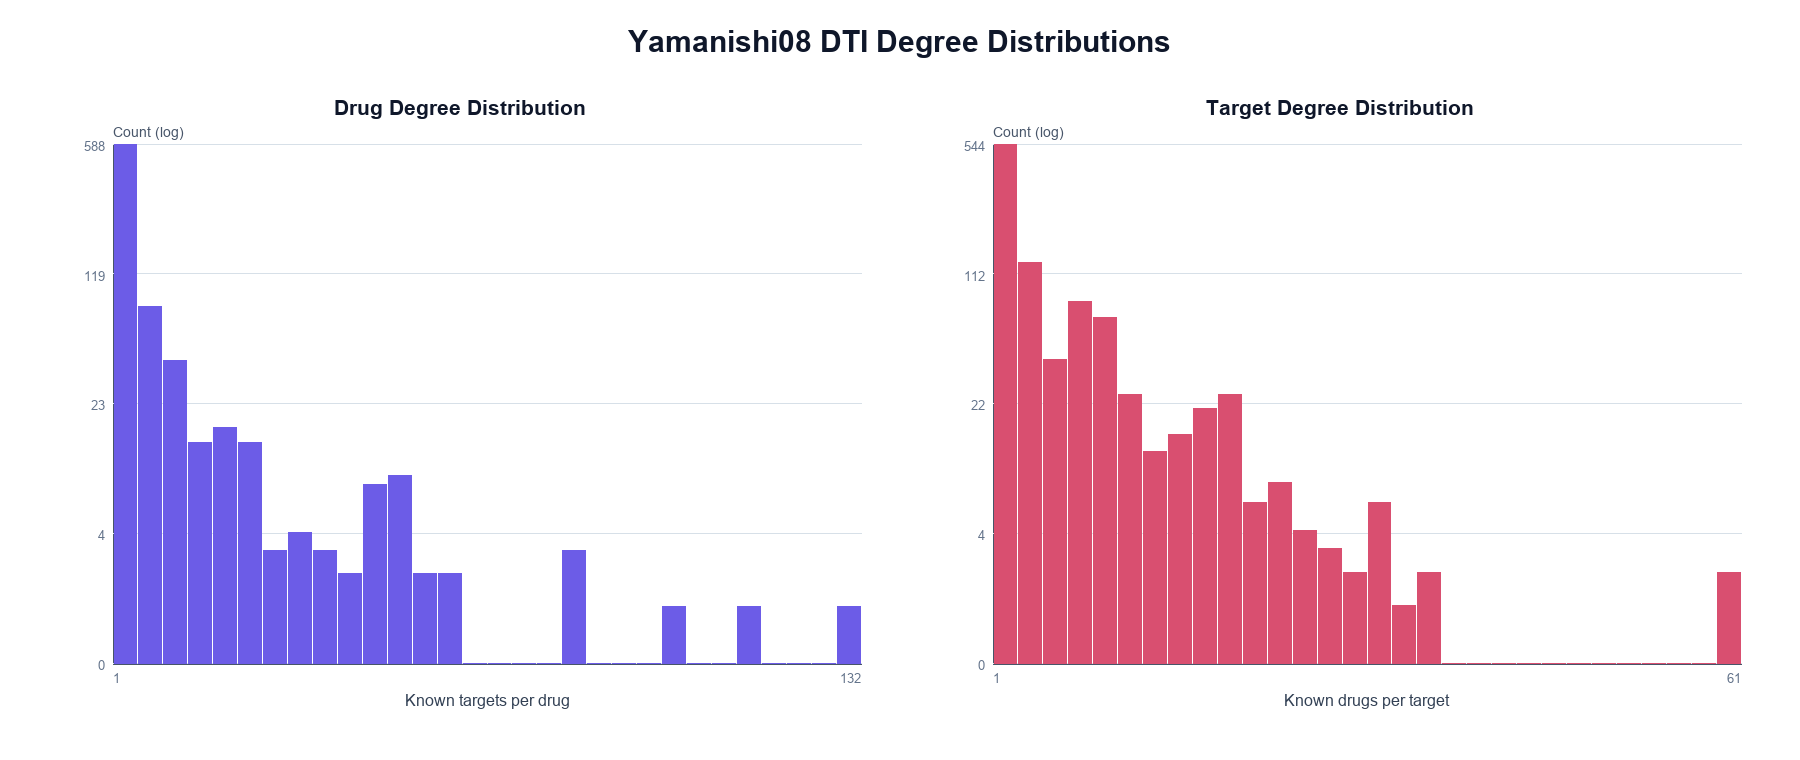
\includegraphics[width=0.9\textwidth]{images/data_analysis/dti_degree_distribution.png}
    \caption{Degree distributions of drugs and targets in the Yamanishi08 DTI network. The log-scale counts show that most entities have few known interactions, while a small number of drugs and targets act as high-degree hubs.}
    \Description{Two log-scale histograms showing known targets per drug and known drugs per target in the Yamanishi08 DTI network, with many low-degree entities and a few high-degree hubs.}
    \label{fig:dti_degree_distribution}
\end{figure*}
The experiments use the Yamanishi08 benchmark for drug--target interaction prediction. The DTI network contains 5,127 known positive interactions between 791 drugs and 989 target proteins. These positives occupy only 0.6554\% of the 782,299 possible drug--target pairs, so the task is sparse at the interaction level. Unobserved pairs are sampled as negatives for training and evaluation, but they are not experimentally confirmed non-interactions.

\begin{table}[t]
\centering
\caption{Key statistics of the Yamanishi08 DTI data and auxiliary knowledge graph.}
\label{tab:dataset_stats}
\small
\begin{tabular}{lr}
\toprule
\textbf{Statistic} & \textbf{Value} \\
\midrule
Known positive interactions & 5,127 \\
Unique drugs & 791 \\
Unique target proteins & 989 \\
Possible drug--target pairs & 782,299 \\
Observed positive density & 0.6554\% \\
Average targets per drug & 6.48 \\
Average drugs per target & 5.18 \\
Auxiliary KG triples & 95,579 \\
Auxiliary KG entities & 25,487 \\
Auxiliary KG relation types & 48 \\
\bottomrule
\end{tabular}
\end{table}

Each drug is represented by a 1,024-dimensional Morgan fingerprint and each protein by a 147-dimensional CTD descriptor. The auxiliary knowledge graph covers all evaluated drugs and targets, providing 95,579 unique biomedical triples over 25,487 entities and 48 relation types. The warm-start protocol evaluates unseen drug--target pairs while keeping test drugs and proteins present in training.


Figure~\ref{fig:dti_degree_distribution} shows that the interaction evidence is also long-tailed at the entity level. Most drugs and targets have only a few known interactions, while a small number of hubs have many. In the underlying statistics, 74.3\% of drugs have at most five known targets and 55.0\% of targets have at most two known drugs.

This structure motivates models that do not rely only on direct DTI frequency. KG embeddings can provide graph-derived context for low-degree drugs and targets, and CompGCN-style message passing can propagate information through typed biomedical relations before the downstream NFM combines graph, molecular, and sequence features.

% !TEX root = ../Report.tex
\section{Methodology}
\label{sec:methodology}
\begin{figure*}[t]
\centering

\includegraphics[width=0.82\textwidth]{images/chapter5_overall_architecture.pdf}
\caption{KGE-NFM framework with alternative DistMult and CompGCN encoders. The KG encoder produces drug and protein embeddings that are combined with molecular and sequence descriptors before NFM prediction.}
\Description{A pipeline from biomedical knowledge graph to DistMult or CompGCN encoder, drug and protein embeddings, descriptor features, neural factorization machine, and DTI probability.}
\label{fig:kge_nfm_architecture}
\end{figure*}

\subsection{Framework Overview}

The proposed methodology follows the KGE-NFM paradigm for DTI prediction, in which relational biomedical evidence is first encoded at the entity level and then integrated with intrinsic drug and protein descriptors for supervised pair classification. The central design choice in this study is the knowledge graph encoder. The original KGE-NFM formulation uses DistMult to obtain drug and protein embeddings, whereas this work evaluates whether replacing that bilinear encoder with CompGCN improves the representations supplied to the downstream predictor. All other stages, including fold construction, descriptor processing, feature-field design, and the NFM classifier, are held fixed so that the comparison focuses on the effect of the KG representation model.

As shown in Figure~\ref{fig:kge_nfm_architecture}, the framework is trained sequentially rather than end-to-end. For each fold, the KG encoder is trained on supporting biomedical triples together with the positive DTI triples from the training split; test DTI labels are excluded from graph construction. The trained encoder then provides separate graph-derived embeddings for the drug and protein in each candidate pair. These embeddings are treated as complementary context features, not as replacements for entity descriptors. The final predictor therefore receives four aligned fields: drug KG embedding, protein KG embedding, drug Morgan fingerprint, and protein CTD descriptor. NFM projects these heterogeneous fields into a shared latent space and learns their pairwise and nonlinear interactions before producing the DTI probability.


\subsection{Problem Formulation and Training Graph}

For a drug $d$ and protein $p$, KGE-NFM estimates
\begin{equation}
    \hat{y}_{dp}=F(d,p),
\end{equation}
where $\hat{y}_{dp}\in[0,1]$ is the predicted interaction probability and the supervised label is $y_{dp}\in\{0,1\}$. The KGE stage learns representations through an encoder $g_{\theta}$:
\begin{equation}
    \mathbf{z}_{d}=g_{\theta}(d,\mathcal{G}),
    \qquad
    \mathbf{z}_{p}=g_{\theta}(p,\mathcal{G}),
\end{equation}
where $g_{\theta}$ is instantiated as either DistMult or CompGCN. The NFM stage then predicts
\begin{equation}
    \hat{y}_{dp}
    =
    \operatorname{NFM}
    \left(
        \mathbf{z}_{d},
        \mathbf{z}_{p},
        \mathbf{s}_{d},
        \mathbf{s}_{p}
    \right),
\end{equation}
with drug descriptor $\mathbf{s}_{d}$ and protein descriptor $\mathbf{s}_{p}$.

For each cross-validation fold, the KGE training graph is constructed as
\begin{equation}
    \mathcal{T}_{train}^{KGE}
    =
    \mathcal{T}_{support}
    \cup
    \mathcal{T}_{DTI,train}^{+}.
    \label{eq:kge_training_graph}
\end{equation}
Here, $\mathcal{T}_{support}$ denotes biomedical context triples such as pathway, annotation, domain, family, and interaction relations, while $\mathcal{T}_{DTI,train}^{+}$ contains only positive DTI triples from the training split. Negative triples are generated by corrupting heads or tails, and both KGE encoders use the margin-ranking objective in Equation~\ref{eq:background_kge_loss}. Feature scaling and optional PCA are fitted on training data and then applied to test data to prevent leakage.

\subsection{DistMult Encoder}

DistMult assigns a vector to each entity and relation \cite{yang2015embedding}. For a triple $(h,r,t)$,
\begin{equation}
    \mathbf{h},\mathbf{r},\mathbf{t}
    \in
    \mathbb{R}^{k}.
\end{equation}
The triple score is a diagonal bilinear interaction:
\begin{equation}
    f_{\mathrm{DM}}(h,r,t)
    =
    \mathbf{h}^{\top}
    \operatorname{diag}(\mathbf{r})
    \mathbf{t}
    =
    \sum_{i=1}^{k}h_i r_i t_i.
    \label{eq:distmult_score}
\end{equation}
This form is efficient because it avoids a full relation-specific matrix. After KGE training, drug and protein representations are read from the learned entity embedding table:
\begin{equation}
    \mathbf{z}_{d}^{DM}=\mathbf{E}[d],
    \qquad
    \mathbf{z}_{p}^{DM}=\mathbf{E}[p].
\end{equation}

DistMult is a useful baseline, but its score is symmetric for a fixed relation:
\begin{equation}
    f_{\mathrm{DM}}(h,r,t)
    =
    f_{\mathrm{DM}}(t,r,h).
\end{equation}
It also learns through triple-level scoring rather than explicit neighborhood aggregation. These limitations motivate the CompGCN encoder, which updates entity states using relation-conditioned messages.

\subsection{CompGCN Encoder}

CompGCN is a multi-relational graph convolutional encoder that jointly updates entity and relation representations \cite{vashishth2020composition}. For each original triple $(u,r,v)$, the graph is augmented with an inverse triple $(v,r^{-1},u)$ and self-loop relations. Original, inverse, and self-loop edges allow information to propagate with direction-aware semantics. At layer $k$, CompGCN maintains entity states $\mathbf{h}_{v}^{k}$ and relation states $\mathbf{h}_{r}^{k}$.

Before aggregation, a neighboring entity representation is composed with the relation embedding:
\begin{equation}
    \mathbf{m}_{u,r}^{k}
    =
    \phi
    \left(
        \mathbf{h}_{u}^{k},
        \mathbf{h}_{r}^{k}
    \right).
\end{equation}
The supported composition functions are subtraction, element-wise multiplication, and circular correlation:
\begin{align}
    \phi_{sub}(\mathbf{h}_{u},\mathbf{h}_{r})
    &=
    \mathbf{h}_{u}-\mathbf{h}_{r}, \\
    \phi_{mult}(\mathbf{h}_{u},\mathbf{h}_{r})
    &=
    \mathbf{h}_{u}\odot\mathbf{h}_{r}, \\
    \phi_{corr}(\mathbf{h}_{u},\mathbf{h}_{r})
    &=
    \mathbf{h}_{u}\star\mathbf{h}_{r}.
\end{align}
Here, $\odot$ denotes element-wise multiplication and $\star$ denotes circular correlation. The main configuration uses multiplication, so messages are relation-gated as
\begin{equation}
    \phi
    \left(
        \mathbf{h}_{u}^{k},
        \mathbf{h}_{r}^{k}
    \right)
    =
    \mathbf{h}_{u}^{k}\odot\mathbf{h}_{r}^{k}.
\end{equation}

The node update aggregates composed messages:
\begin{equation}
    \mathbf{h}_{v}^{k+1}
    =
    \sigma
    \left(
        \sum_{(u,r)\in\mathcal{N}(v)}
        \mathbf{W}_{\lambda(r)}^{k}
        \phi
        \left(
            \mathbf{h}_{u}^{k},
            \mathbf{h}_{r}^{k}
        \right)
    \right),
    \label{eq:compgcn_node_update}
\end{equation}
where $\mathcal{N}(v)$ is the relational neighborhood of $v$, $\sigma$ is a nonlinear activation, and $\lambda(r)\in\{O,I,S\}$ selects transformations for original, inverse, and self-loop edges. Thus, CompGCN shares direction-specific matrices $\mathbf{W}_{O}^{k}$, $\mathbf{W}_{I}^{k}$, and $\mathbf{W}_{S}^{k}$ rather than learning a separate full transformation for every relation. Relation embeddings are updated as
\begin{equation}
    \mathbf{h}_{r}^{k+1}
    =
    \mathbf{W}_{rel}^{k}
    \mathbf{h}_{r}^{k}.
    \label{eq:compgcn_relation_update}
\end{equation}
Stacking $L$ layers yields entity states $\mathbf{h}_{v}^{L}$ that encode relation-conditioned neighborhood information. Figure~\ref{fig:compgcn_message_passing} illustrates this message-passing mechanism.

\begin{figure}[t]
\centering

\includegraphics[width=\columnwidth]{images/chapter5_compgcn_message_passing.pdf}
\caption{CompGCN message passing. Neighboring entity states are composed with relation states and transformed according to edge direction before aggregation.}
\Description{A CompGCN message-passing diagram showing original, inverse, and self-loop relation-aware messages flowing into an entity update.}
\label{fig:compgcn_message_passing}
\end{figure}

CompGCN acts as an encoder whose enriched entity and relation states are passed to a link-prediction decoder:
\begin{equation}
    f_{CG}(h,r,t)
    =
    \operatorname{Dec}
    \left(
        \mathbf{h}_{h}^{L},
        \mathbf{h}_{r}^{L},
        \mathbf{h}_{t}^{L}
    \right).
\end{equation}
The encoder--decoder model is optimized with the same negative-sampling and margin-ranking setup used for DistMult. After training, the enriched drug and protein embeddings are extracted as
\begin{equation}
    \mathbf{z}_{d}^{CG}=\mathbf{h}_{d}^{L},
    \qquad
    \mathbf{z}_{p}^{CG}=\mathbf{h}_{p}^{L}.
\end{equation}
These vectors replace the DistMult embeddings in the downstream NFM while leaving the rest of the pipeline unchanged.

\subsection{Feature Construction}

For either encoder, the candidate pair contains four feature fields:
\begin{equation}
    \mathcal{F}_{dp}
    =
    \left\{
        \mathbf{z}_{d},
        \mathbf{z}_{p},
        \mathbf{s}_{d},
        \mathbf{s}_{p}
    \right\}.
    \label{eq:kge_nfm_fields}
\end{equation}
The graph fields $\mathbf{z}_{d}$ and $\mathbf{z}_{p}$ represent relational biomedical context. The descriptor fields are a 1024-dimensional Morgan fingerprint $\mathbf{s}_{d}\in\mathbb{R}^{1024}$ and a 147-dimensional protein CTD descriptor $\mathbf{s}_{p}\in\mathbb{R}^{147}$. Conceptually, the pair representation is
\begin{equation}
    \mathbf{x}_{dp}
    =
    [
        \mathbf{z}_{d}
        \mathbin{\Vert}
        \mathbf{z}_{p}
        \mathbin{\Vert}
        \mathbf{s}_{d}
        \mathbin{\Vert}
        \mathbf{s}_{p}
    ],
\end{equation}
but the implemented NFM processes the four blocks as separate fields. This preserves the distinction between drug graph context, protein graph context, molecular structure, and protein sequence descriptors.

\subsection{Neural Factorization Machine}

The downstream predictor is a field-based NFM derived from the NFM principle in \cite{he2017neural}. Each input field $\mathbf{x}_{dp}^{(m)}\in\mathbb{R}^{D_m}$ is projected into a shared latent dimension:
\begin{equation}
    \mathbf{u}_{m}
    =
    \mathbf{P}_{m}\mathbf{x}_{dp}^{(m)}+\mathbf{b}_{m}.
    \label{eq:nfm_field_projection}
\end{equation}
The projected fields are combined using Bi-Interaction pooling:
\begin{equation}
    \mathbf{f}_{BI}
    =
    \frac{1}{2}
    \left[
        \left(
            \sum_{m=1}^{M}\mathbf{u}_{m}
        \right)^2
        -
        \sum_{m=1}^{M}\mathbf{u}_{m}^{2}
    \right].
    \label{eq:nfm_bi_interaction}
\end{equation}
This operation summarizes pairwise interactions among the four fields. The pooled vector is then processed by hidden layers:
\begin{equation}
    \mathbf{a}^{(l+1)}
    =
    \operatorname{ReLU}
    \left(
        \mathbf{W}^{(l)}\mathbf{a}^{(l)}+\mathbf{b}^{(l)}
    \right),
    \qquad
    \mathbf{a}^{(0)}=\mathbf{f}_{BI}.
\end{equation}

The final logit combines field-level linear terms and the nonlinear interaction network:
\begin{equation}
    o_{dp}
    =
    \sum_{m=1}^{M}
    \left(
        \mathbf{a}_{m}^{\top}\mathbf{x}_{dp}^{(m)}+c_m
    \right)
    +
    \operatorname{MLP}(\mathbf{f}_{BI}).
\end{equation}
The predicted DTI probability is
\begin{equation}
    \hat{y}_{dp}=\operatorname{sigmoid}(o_{dp}).
\end{equation}
NFM is optimized with binary cross-entropy:
\begin{equation}
    \mathcal{L}_{DTI}
    =
    -\frac{1}{N}
    \sum_{i=1}^{N}
    \left[
        y_i\log(\hat{y}_i)
        +(1-y_i)\log(1-\hat{y}_i)
    \right].
\end{equation}
This final stage is where relational embeddings and descriptor fields are jointly converted into an interaction probability.

% !TEX root = ../Report.tex
\section{Experiments and Results}
\label{sec:results}

\subsection{Experimental Setup}

Experiments are conducted on the Yamanishi08 DTI benchmark under two warm-start class-ratio settings: Yamanishi 1:1 and Yamanishi 1:10. Each setting contains ten supplied folds, and the same folds are used for descriptor baselines and KGE-NFM variants so that average ROC-AUC and PR-AUC values are directly comparable. The 1:10 setting is used for CompGCN tuning because it is the more imbalanced and practically demanding ranking condition.

The classical baselines use the 1,024-dimensional Morgan fingerprint for each drug and the protein CTD descriptor. In the KGE-NFM pipeline, fold-specific entity embeddings are learned from the training knowledge graph and combined with descriptor fields in the downstream NFM. DistMult and CompGCN are evaluated as alternative KGE encoders, while the NFM architecture and evaluation protocol are kept fixed. The selected CompGCN configuration uses 200-dimensional embeddings, 50 KGE training epochs, five negative samples per positive triple, three CompGCN layers, element-wise multiplication composition, dropout 0.1, and NFM hidden layers of 128 and 128 units trained for up to 200 epochs with early stopping. The protein CTD block is reduced to 100 PCA components.

\subsection{Baselines and Metrics}

The compared methods are Logistic Regression, Random Forest, XGBoost, DistMult-NFM, and CompGCN-NFM. Logistic Regression provides a linear descriptor-only reference; Random Forest and XGBoost are nonlinear descriptor baselines; DistMult-NFM measures the effect of conventional KGE embeddings; and CompGCN-NFM tests whether relation-aware message passing improves the embeddings supplied to NFM.

ROC-AUC measures ranking discrimination across thresholds, i.e., the probability that a randomly selected positive pair is ranked above a randomly selected negative pair. PR-AUC summarizes precision--recall behavior and is especially important for Yamanishi 1:10, where sampled negatives are much more frequent than positives.

\subsection{Main Results}
\label{sec:main_results}

\begin{table}[!htbp]
\centering
\caption{Average DTI prediction performance on Yamanishi08 warm-start settings.}
\label{tab:main_results}
\small
\setlength{\tabcolsep}{3pt}
\resizebox{\columnwidth}{!}{%
\begin{tabular}{lcccc}
\toprule
& \multicolumn{2}{c}{\textbf{Yamanishi 1:1}} &
\multicolumn{2}{c}{\textbf{Yamanishi 1:10}} \\
\cmidrule(lr){2-3}\cmidrule(lr){4-5}
\textbf{Model} & \textbf{ROC-AUC} & \textbf{PR-AUC} &
\textbf{ROC-AUC} & \textbf{PR-AUC} \\
\midrule
Logistic Regression & 0.7139 & 0.6613 & 0.7255 & 0.1726 \\
Random Forest       & 0.9024 & 0.9014 & 0.9486 & 0.7743 \\
XGBoost             & 0.9051 & 0.8948 & 0.9225 & 0.6198 \\
DistMult-NFM        & 0.9413 & 0.9390 & 0.9804 & 0.9315 \\
CompGCN-NFM         & \textbf{0.9689} & \textbf{0.9681} &
                      \textbf{0.9866} & \textbf{0.9362} \\
\bottomrule
\end{tabular}
}
\end{table}

Table~\ref{tab:main_results} reports the average performance over the ten supplied folds. CompGCN-NFM obtains the best value in all four metric columns. On Yamanishi 1:1, it improves over DistMult-NFM by 0.0276 ROC-AUC and 0.0291 PR-AUC. On Yamanishi 1:10, the gains are smaller but remain positive, at 0.0063 ROC-AUC and 0.0047 PR-AUC.

The strongest descriptor-only baseline on Yamanishi 1:10 is Random Forest, with 0.9486 ROC-AUC and 0.7743 PR-AUC. CompGCN-NFM improves these values by 0.0380 and 0.1619, respectively. The larger PR-AUC gain is important because PR-AUC is more sensitive to false positives in the imbalanced setting. Both KGE-NFM variants outperform the descriptor baselines, indicating that graph-derived features add useful relational context beyond Morgan fingerprints and CTD descriptors.

\subsection{Hyperparameter Tuning}
\label{sec:hyperparameter_tuning}

\begin{table}[!htbp]
\centering
\caption{CompGCN hyperparameter tuning results on Yamanishi 1:10.}
\label{tab:compgcn_tuning}
\small
\begin{tabularx}{\columnwidth}{Xcc}
\toprule
\textbf{Recorded configuration} & \textbf{ROC-AUC} & \textbf{PR-AUC} \\
\midrule
Embedding dimension 200 & 0.986336 & 0.932113 \\
Embedding dimension 400 & 0.980704 & 0.889596 \\
Embedding dimension 600 & 0.965040 & 0.839139 \\
Embedding 200, 3 negatives & 0.985824 & 0.932002 \\
Embedding 200, 5 negatives & 0.986321 & 0.933304 \\
Embedding 200, 5 negatives, 1 layer & 0.985215 & 0.927070 \\
Embedding 200, 5 negatives, 3 layers & \textbf{0.986632} & \textbf{0.936223} \\
\bottomrule
\end{tabularx}
\end{table}

Table~\ref{tab:compgcn_tuning} reports the staged CompGCN tuning experiments on Yamanishi 1:10. The search varies embedding dimension, number of negative samples, and number of message-passing layers while keeping other settings at their run defaults.

The results favor 200-dimensional embeddings. Increasing the dimension to 400 or 600 reduces both metrics, suggesting that additional capacity does not improve this graph and training setup. With the embedding dimension fixed at 200, five negative samples outperform three in PR-AUC, and three CompGCN layers outperform one layer.

\subsection{Ablation Study}
\label{sec:ablation_study}

\begin{table}[!htbp]
\centering
\caption{Ablation results on Yamanishi 1:10.}
\label{tab:ablation_study}
\small
\setlength{\tabcolsep}{3pt}
\resizebox{\columnwidth}{!}{%
\begin{tabular}{lrrrr}
\toprule
\textbf{Configuration} & \textbf{ROC-AUC} & \textbf{PR-AUC} &
\textbf{$\Delta$ ROC vs. full} & \textbf{$\Delta$ PR vs. full} \\
\midrule
KGE only & 0.619957 & 0.145284 & $-0.366675$ & $-0.790939$ \\
NFM only, without KGE dense embeddings & 0.929957 & 0.845284 & $-0.056675$ & $-0.090939$ \\
Without Morgan and protein descriptors & 0.969570 & 0.922840 & $-0.017062$ & $-0.013383$ \\
Full CompGCN-NFM & \textbf{0.986632} & \textbf{0.936223} & 0.000000 & 0.000000 \\
\bottomrule
\end{tabular}
}
\end{table}

Table~\ref{tab:ablation_study} evaluates the selected CompGCN configuration on Yamanishi 1:10 and separates the contribution of graph scoring, descriptor-based NFM prediction, dense KGE embeddings, and the complete multimodal pipeline. The full CompGCN-NFM result from Table~\ref{tab:main_results} is included as the reference configuration.

The standalone KGE scorer performs poorly, particularly in PR-AUC, showing that graph scoring alone is insufficient for the final binary DTI task. The descriptor-based NFM without dense KGE embeddings is much stronger, reaching 0.929957 ROC-AUC and 0.845284 PR-AUC, but it still trails the full model by 0.056675 ROC-AUC and 0.090939 PR-AUC. Removing Morgan and CTD descriptors causes a smaller reduction, indicating that graph embeddings and NFM feature interactions account for most of the performance, while molecular and sequence descriptors provide complementary gains.

\subsection{Discussion and Limitations}

The main empirical finding is the consistent ordering of average scores: CompGCN-NFM performs best, followed by DistMult-NFM, while descriptor-only baselines remain behind the KGE-enhanced models. This supports the methodological motivation for relation-aware graph encoding, but the improvement over DistMult is modest in the harder Yamanishi 1:10 setting. Therefore, the evidence supports a cautious claim: CompGCN provides useful additional relational context, but the magnitude of the gain should be interpreted with fold-level variability and statistical testing when those values are available.

The results also show why both ROC-AUC and PR-AUC are needed. Several models retain high ROC-AUC under the 1:10 setting, but descriptor baselines lose substantial PR-AUC as the negative class grows. The KGE-NFM variants preserve much higher PR-AUC, suggesting better positive-ranking behavior under imbalance. Limitations remain: the current summary reports fold averages rather than confidence intervals, tuning is staged rather than exhaustive, sampled negatives may include unknown true interactions, and warm-start evaluation does not test generalization to entirely unseen drugs or proteins.

% !TEX root = ../Report.tex
\section{Conclusion}
\label{sec:conclusion}

This report presented a KGE-NFM study for DTI prediction. The pipeline learns fold-specific drug and protein embeddings from a biomedical KG, combines them with Morgan fingerprints and protein CTD descriptors, and predicts interactions with an NFM classifier. DistMult and CompGCN were evaluated as alternative graph encoders under the same downstream protocol.

The experimental results on Yamanishi08 show that KG-enhanced NFM models outperform descriptor-only baselines, and that CompGCN-NFM gives the strongest average performance. The model reaches 0.9689 ROC-AUC and 0.9681 PR-AUC on Yamanishi 1:1, and 0.9866 ROC-AUC and 0.9362 PR-AUC on Yamanishi 1:10. Ablation results further show that standalone graph scoring is insufficient, while the full model benefits from combining graph-derived embeddings with molecular and sequence descriptors.

Future work should add fold-level confidence intervals and paired statistical tests, evaluate drug-cold-start and protein-cold-start settings, and compare additional KGE encoders such as ComplEx, RotatE, and TransE under the same NFM protocol. Richer drug and protein representations, including molecular graph neural networks and protein language models, may also improve generalization beyond the current descriptor blocks.


\bibliographystyle{ACM-Reference-Format}
\bibliography{Refs/references}

\end{document}
